\documentclass[]{article}
\usepackage{polyglossia}
\usepackage{fancyhdr}
\usepackage{enumerate}
\usepackage{framed}
\usepackage{listings}
\usepackage{amsfonts}
\usepackage[usenames,dvipsnames,svgnames,table]{xcolor}
\usepackage{minted}
\usepackage{hyperref}
\usepackage{graphicx}
\usepackage{gensymb}
\usepackage{diagbox}
\graphicspath{ {./images/} }

\setmainlanguage{spanish}
\definecolor{mygray}{RGB}{248,249,250}

\newcommand{\pythonblock}{\inputminted[linenos,bgcolor=mygray,framesep=10pt,firstnumber=\value{pythonnumber}]{python3}}
\newcommand{\asw}{\textbf{R. }}
\renewcommand{\theFancyVerbLine}{\sffamily \textcolor[rgb]{0.5,0.5,1.0}{\footnotesize \oldstylenums{\arabic{FancyVerbLine}}}}

\title{Evaluación Nº3 \protect\\ Algoritmos y programación}
\author{Anggelo Urso G. \\ anggelo.urso@inacapmail.cl}
\date{\today}

\pagestyle{fancy}
\fancyhf{}
\lhead{Algoritmos y programación}
\rhead{\thepage}
\lfoot{AUG /\LaTeX}
\rfoot{
\includegraphics[scale=0.4]{cc-lic}}

\hypersetup{
    colorlinks=true,
    linkcolor=blue,
    filecolor=magenta,      
    urlcolor=cyan,
}

\newcounter{pythonnumber}
\setcounter{pythonnumber}{1}

\begin{document}
    \thispagestyle{empty}
    \maketitle

    \section{Introducción}

    \section{Descripción del problema}
    Dado a que el tradicional juego del piedra/papel/tijera presenta una cantidad significativa de posibles empates, existe una variante bastante interesante para aumentar el número de combinaciones y así reducir la cantidad de empates que se puedan generar.

    El juego se llama piedra/papel/tijera/lagarto/spock\footnote{Agradecimientos a The Big Bang Theory, capítulo donde se explica el juego \href{https://www.youtube.com/watch?v=43ijRL7w8z8}{https://www.youtube.com/watch?v=43ijRL7w8z8}}. La idea de la actividad es que logren programar el juego, utilizando para ello el lenguaje de programación en C. Éste podrá ser jugado a través de las siguientes modalidades:

    \begin{enumerate}
        \item Jugador vs Computador
        \item Jugador vs Jugador
    \end{enumerate}

    El alumno deberá programar el juego, entregando las opciones correspondientes al jugador o los jugadores y evaluar: quien ha sido el ganador, quien pierde o si hubo empate.

    \section{Reglas del juego}
    Tal como el tradicional juego piedra/papel/tijera, dependiendo de la opción se evalúan los resultados de acuerdo a la siguiente tabla.\\

    \begin{center}    
        \begin{tabular}{|l|c|c|c|c|c|}
            \hline
            \diagbox{Jugador 1}{Jugador 2}& Piedra & Papel & Tijera & Lagarto & Spock \\
            \hline\hline
            Piedra & E & - & X & X & - \\
            \hline
            Papel & X & E & - & - & X \\
            \hline
            Tijera & - & X & E & X & - \\
            \hline
            Lagarto & - & X & - & E & X \\
            \hline
            Spock & X & - & X & - & E \\
            \hline
        \end{tabular}
    \end{center}

    En esta tabla se puede observar las combinaciones de empates (\textbf{E}), cuando el jugador 1 gana (\textbf{X}) y cuando el jugador 2 gana (\textbf{-}). Cuando se juega contra la computadora, el jugador escoge una de las alternativas y el computador escoge otra de forma aleatoria.

    Para simplificar el problema se utilizarán tiradas secuenciales, es decir, el jugador 1 escogerá su opción y luego el jugador 2. En el caso de jugar contra la computadora, el jugador 1 realizará su tirada y el computador escogerá una de las alternativas disponibles de forma aleatoria.

    Al final de la tirada, se deberá desplegar quien es el jugador que gana (o si gana la computadora). Si se juega contra la computadora, el programa deberá indicar cuál es la tirada que escogió la computadora e indicar el resultado.

    \section{Restricciones del problema}
    Como restricciones del juego, deberán considerar que las opciones a ser ingresadas deberán presentarse en un menú de opciones a los jugadores, cada uno de ellos escogerá una de las 5 opciones, o decidirán volver a la pantalla anterior. Para esto podrán utilizar la siguiente imagen como referencia:

    \begin{figure}[H]
        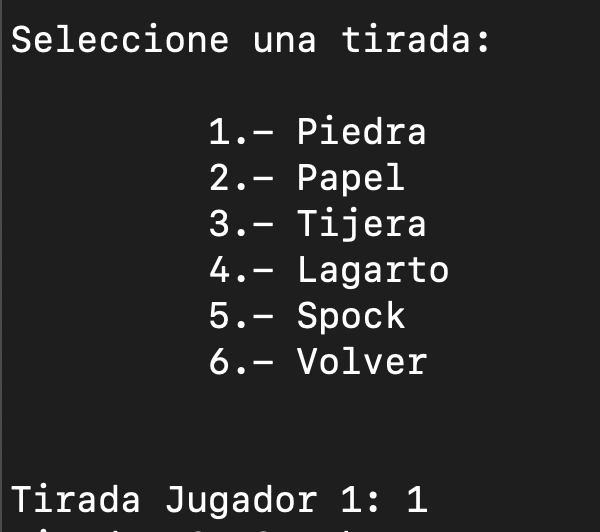
\includegraphics[scale=0.5]{ejMenuJugador}
    \end{figure}

    Si observan, cada una de las opciones está mapeada con un número, incluyendo la opción volver, que redirige a cualquiera de los dos jugadores a la pantalla inicial:

    \begin{figure}[H]
        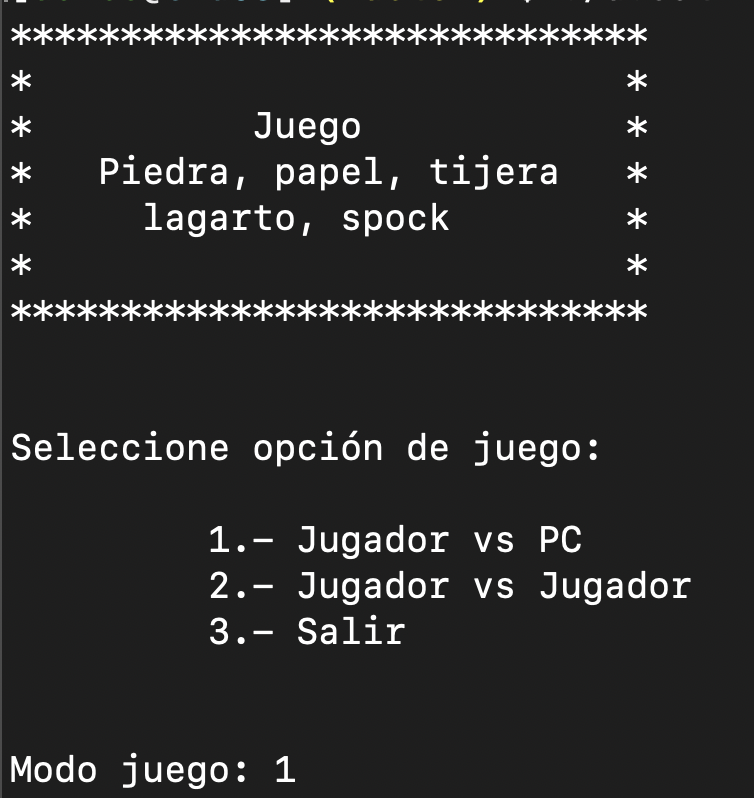
\includegraphics[scale=0.5]{ejPantallaInicial}
        \label{img.2}
    \end{figure}

    Acá si observan, tienen las tres opciones: Jugador vs computadora, jugador vs jugador y salir; la cual termina la ejecución del programa. Como datos de entrada deberán ingresar un número de dicho menú para ir navegando.

    Otra de las restricciones, es la utilización de la función random. Para eso deberán incluir el siguiente código:\\

    \begin{listing}[H]
        \begin{minted}[linenos,bgcolor=mygray,framesep=10pt]{C}
#include <stdio.h> // para usar printf y scanf
#include <stdlib.h> // para usar rand y srand
#include <unistd.h> // para getpid()

int main() {
    srand(getpid()); // genera una semilla aleatoria
    int numero = rand() % 5; // genera un random en el anillo
    return 0;
}
        \end{minted}
        \label{code.1}
    \end{listing}

    La función \textbf{srand(getpid())} puede en cualquier parte del código, pero recomiendo que la dejen en el \textbf{main} del programa, así la función \textbf{rand()} tendrá acceso a la semilla aleatoria en cualquier parte del programa que lo definan.

    El programa no deberá terminar hasta que no se seleccione la opción 3 del menu de juego (Salir). Hasta antes de eso, el jugador podrá ir seleccionando distintas modalidades de juego.

    La cabecera presentada en la imagen \ref{img.2}, es meramente referencial y no es necesario dejar una cabecera similar o incluirla en el desarrollo de la actividad.

    \section{Restricciones de la evaluación}
    Para la presente evaluación y en línea con los objetivos planteados al comienzo del documento, se espera que los alumnos entreguen un trabajo con las siguientes restricciones:

    \begin{enumerate}
        \item Se deberá entregar un archivo fuente (formato \textbf{.c}) que permita ejecutar su programa.
        \item Deberá respetar el formato de entrada de datos (solo enteros).
        \item Deberá contar con a lo menos 1 función y a lo menos 2 ciclos.
        \item Deberán necesariamente utilizar las librerías descritas en el segmento de código \ref{code.1}.
        \item Deberán utilizar las funciones \textbf{rand} para la tirada de la computadora, de manera que sea una elección aleatoria.
        \item La compilación no deberá proporcionar ningún tipo de error o advertencia.
        \item No es obligatorio que los mismos alumnos que entregaron la evaluación 2 como equipo, entreguen la evaluación 3. Los equipos puede mutar o pueden decidir hacer la actividad de forma individual.
    \end{enumerate}

    \section{Fecha de entrega y formato}
    Se establece como fecha de entrega de la evaluación 3, el día lunes 27 de julio, antes de las 23:55 hrs.
    
    Solo será necesario que entreguen el archivo 1 de los miembros del equipo de trabajo, indicando a través de un comentario multilínea los integrantes y respetando el siguiente formato:\\

    \begin{listing}[H]
        \begin{minted}[linenos,bgcolor=mygray,framesep=10pt]{C}
/*
    Evaluación 2 - Algoritmos y programación
    Integrantes:
        - Nombre alumno 1 - Rut alumno 1
        - Nombre alumno 2 - Rut alumno 2
    Sección: Nº sección
*/
        \end{minted}
    \end{listing}

    En caso de que el trabajo sea realizado de forma individual, se deberá respetar el formato anterior, pero indicando solo al alumno que lo realizó.

    El formato de entrega será un archivo fuente C (extensión \textbf{C}) que deberá ser subido al ambiente de aprendizaje antes de la fecha indicada anteriormente. 

    \textbf{Importante:} Bajo ningún punto se recibirán trabajos fuera de fecha o a través de otro medio que no sea el indicado anteriormente (AAI). Cualquier trabajo que no respete el formato indicado en la evaluacn o fuera de fecha \textbf{no será revisado}. 
\end{document}